
Given the results of
direct simulation it is
possible to examine
the limitations
and success of the
Lindblad analysis.

\subsection{Separable Density matrix}

\subsection{Diagonal Electron Density Matrix}
In \ldots we make the approximation
TODO- How big are the off diagonal elements??

\subsection{Single State Tunnelling Rate}\label{sec:lindblad corrected tunneling}
When simulating the
degenerate hydrogen tunneling in
\cref{sec:degenerate tunnelling simulaton}
we found that the tunneling rate
grew proportional to \(4R_0N(1-N)\).
This corresponds exactly to the
form of the integrand of
\cref{eqn:gamma integral form},
which was proportional to
\(N_1(1 - N_3)\) where
\(E_{k3} = E_{k1} + \omega{}\),
and \(\omega{}\) is equal to
the difference in hydrogen energies
\begin{equation}
    \Gamma_{i,j, k,l}(\omega)  =\begin{aligned}[t]
        4 \int &
        \frac{d^3\vec{k}_1}{{(2\pi)}^3}
        \frac{d^3\vec{k}_3}{{(2\pi)}^3}
        V_{i,j} V_{k,l}
        N_1 (1 - N_3)
        \frac{m\delta({k_3 \pm \sqrt{k_1^2 + 2m\omega}})}{\sqrt{k_1^2 - 2m\omega}}
    \end{aligned}
\end{equation}
This suggests
that the process
is dominated
by single electron
transitions, an assumption
that was made in \cref{eqn:second order eqn of motion}
when expanding the equation
of motion to second order.

If we were to look at the
tunneling for \(\omega \neq 0\)
we find that the correct
way to modify the tunneling
rate in the simulation should
be to set
\(R(N\rightarrow{}N') = 2R_0N(1-N')\)
corresponding to \cref{eqn:target correction rate}
in
\cref{sec:corrected transition rate}.


\subsection{Final State Correction}
In \cref{sec:simulation results} we argued
that the electron state immediately
after a transition
should not effect the
dynamics of the system,
however in the Lindblad
analysis it should be possible to
properly take into account
the change in electron
distributions through
the introducing a coupling between
the electron and hydrogen density
matrices.
Although this a difficult
problem in general
if we were
to introduce a coupling
\begin{equation}
    \hat{\rho}_t = \sum_{m,n} \hat{\rho}_{m,n} \otimes {(\hat{\rho}_E)}_{m,n} \
\end{equation}
we can follow the same procedure as in
\cref{sec:the redfield assumption}
to arrive at a modified redfield equation
\begin{equation}
    \bra{m}\dot{\hat{\rho}}(t)\ket{n} = \begin{aligned}[t]
        \sum_{i,j,k, l} &
        \exp{(-i(\omega_{i,j}-\omega_{k,l})t)}
        \Gamma^{m,n}_{i,j;k, l}(\omega_{k,l})
        [S_{k, l}{\hat{\rho}(t)}_{m,n},
        S^\dagger_{i,j}]  \\
        +               &
        \exp{(i(\omega_{i,j}-\omega_{k,l}))}
        {\Gamma^*}^{m,n}_{k, l; i,j}(\omega_{i,j})
        [S_{k, l},
                {\hat{\rho}(t)}_{m,n} S^\dagger_{i,j}]
    \end{aligned}
\end{equation}
where
\begin{equation}
    \Gamma^{m,n}_{i,j, k,l}(\omega) =
    \int_0^\infty{}{
    ds \exp{(i\omega{}s)}
    Tr_{E}[E^\dagger_{i,j}(t)E_{k,l}(t-s)
    {(\hat{\rho}_E)}_{m,n}]
    }
\end{equation}
The problem is then how best to express
both the statistical and quantum uncertainty
in the form of a density matrix.

\subsection{Rotating Wave Approximation}
The final approximation made in
\cref{sec:lindblad equation}
is the rotating wave approximation.
If we relax this approximation
we arrive at the expression
for the full Redfield equation given in
\cref{sec:redfield equation full solution}.
\begin{align}
    \bra{m}\dot{\hat{\rho{}}}(t) \ket{n} & = \begin{aligned}[t]
        \sum_{i,j} &
        \exp{(-i\Delta{}E_{n,j;m,i} t)}
        \Gamma_{n,j;m, i}(\omega_{m,i})
        \rho_{i,j}   \\
                   &
        -\exp{(-i\Delta{}E_{i,m;i,j} t)}
        \Gamma_{i,m;i, j}(\omega_{i,j})
        \rho_{j, n}  \\
                   &
        +\exp{(i\Delta{}E_{n,j;m,i} t)}
        \Gamma_{n,j; m, i}(\omega_{n,j})
        \rho_{i, j}  \\
                   &
        -\exp{(i\Delta{}E_{i,j;i,n} t)}
        \Gamma_{i,j; i, n}(\omega_{i,j})
        \rho_{m, j}
    \end{aligned}
\end{align}
This equation produces extra oscillations
on top of the Lindblad result, with
a characteristic timescales of
\(\frac{2\pi}{\omega_{1,0}} = 2.13\times{}10^{-13}s\). Plotting
the full solution (\cref{fig:redfield full solution})
however we see exactly the same behaviour as that
predicted by the lindblad result.
\begin{figure}[htbp]
    \centering
    \begin{subfigure}{0.45\linewidth}
        \centering
        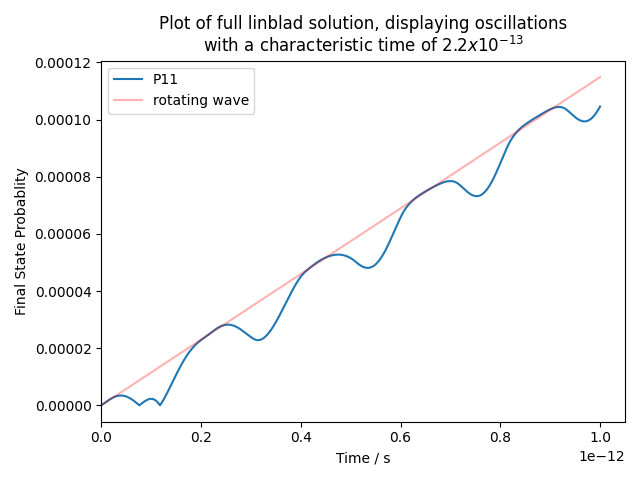
\includegraphics[width =0.9 \linewidth]{Figures/Redfield/Plot of redfield solution short time.png}
        \caption{Complete solution for small times
        }\label{fig:redfield full solution short timescales}
    \end{subfigure}
    \hfill
    \begin{subfigure}{0.45\linewidth}
        \centering
        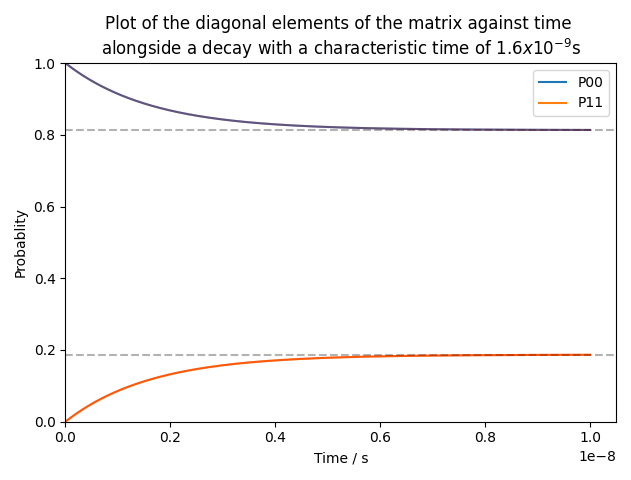
\includegraphics[width = 0.9\linewidth]{Figures/Redfield/Plot of redfield solution long time.png}
        \caption{Complete solution for long times
        }\label{fig:redfield full solution long timescales}
    \end{subfigure}
    \begin{subfigure}{0.45\linewidth}
        \centering
        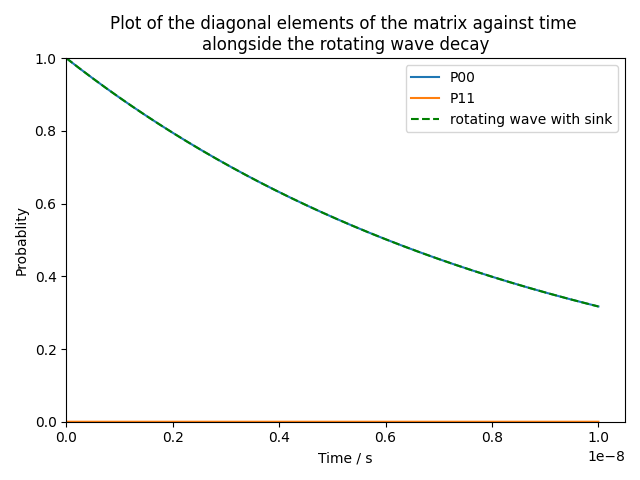
\includegraphics[width = 0.9\linewidth]{Figures/Redfield/Plot of redfield solution long time sink.png}
        \caption{Complete solution with sink
        }\label{fig:redfield full solution with sink}
    \end{subfigure}
    \caption{Plot of the full solution of the Redfield
    equation. On short timescales
    (\cref{fig:redfield full solution short timescales})
    the solution is seen to
    oscillate with a characteristic
    frequency of \(2.1\times{}10^{-13}\)s however
    at long timescales
    (\cref{fig:redfield full solution long timescales})
    the solution decays at the same rate as the
    Lindblad equation. The solution is
    also well behaved with the inclusion of
    a sink at the HCP site
    (\cref{fig:redfield full solution with sink}).
    }\label{fig:redfield full solution}
\end{figure}
In theory we should also be able
to solve the redfield equation
for multiple hydrogen sites, however
the additional computational complexity
rules this out. It is possible to
approximate the behaviour
seen in the many site model
by placing a sink at
the HCP site
(\cref{fig:redfield full solution with sink}).
In this case
we again see good
agreement with the
lindblad equation.